\section{Group Water Systems}\label{group-water-systems}

This group of objects is used to describe the water systems in the building. EnergyPlus offers water modeling capabilities than include not only hot water systems but also the overall water systems including cold water uses, on-site water collection (e.g., from rain, condensate, or well), and storage. HVAC components may consume or collect a significant portion of the water making it appropriate to include water modeling in EnergyPlus.

All water systems are collected into an end use category called Water Systems . This category includes hot and cold water. Water consumed by an HVAC component will be assigned to the end use category for that component. End use subcategories are available to separate hot water from cold water if desired. Simple hot water systems can be configured as stand-alone or use a \hyperref[plantloop]{PlantLoop}. The Water Systems can be connected to \hyperref[plantloop]{PlantLoop}s for modeling heated water end uses. However \hyperref[plantloop]{PlantLoop}s are not used to model cold water and the \hyperref[waterusestorage]{WaterUse:Storage}s portions of the water system. Cold water systems are connected together using \hyperref[waterusestorage]{WaterUse:Storage} objects. \hyperref[wateruseconnections]{WaterUse:Connections} are used at the zone level to connect to both cold and hot water.

In addition to the input objects described in this section below, there are a variety of HVAC components that can be configured to interact with the water systems. These component input objects include optional fields that allow describing how the water systems are connected to them by providing the name of a storage tank. The following table lists EnergyPlus input objects that include provisions for connecting to the water systems but are described elsewhere in this document:

% table 34
\begin{longtable}[c]{p{2.49in}p{3.5in}}
\caption{Water Systems Objects \label{table:water-systems-objects}} \tabularnewline
\toprule
Input Object Name & Type of Water Interactions \tabularnewline
\midrule
\endfirsthead

\caption[]{Water Systems Objects} \tabularnewline
\toprule
Input Object Name & Type of Water Interactions \tabularnewline
\midrule
\endhead

Site:Precipitation & Describes rainfall for WaterUse:RainCollector \tabularnewline
Coil:Cooling:Water & Condensate collection to WaterUse:Storage \tabularnewline
Coil:Cooling:Water:DetailedGeometry & Condensate collection to WaterUse:Storage \tabularnewline
Coil:Cooling:DX:SingleSpeed & Optional evaporative condenser can be supplied by WaterUse:Storage \tabularnewline
Condensate collection to WaterUse:Storage \tabularnewline
Coil:Cooling:DX:TwoSpeed & Evaporative condenser supplied by WaterUse:Storage \tabularnewline
Condensate collection to WaterUse:Storage \tabularnewline
Coil:Cooling:DX:TwoStageWithHumidityControlMode & Evaporative condenser supplied by WaterUse:Storage \tabularnewline
Condensate collection to WaterUse:Storage \tabularnewline
Coil:Cooling:DX:MultiSpeed & Evaporative condenser supplied by WaterUse:Storage \tabularnewline
Condensate collection to WaterUse:Storage \tabularnewline
Humidifier:Steam:Electric & Water supplied by WaterUse:Storage \tabularnewline
CoolingTower:SingleSpeed & Water supplied by WaterUse:Storage \tabularnewline
CoolingTower:TwoSpeed & Water supplied by WaterUse:Storage \tabularnewline
CoolingTower:VariableSpeed & Water supplied by WaterUse:Storage \tabularnewline
ZoneCoolTower:Shower & Water supplied by WaterUse:Storage \tabularnewline
Refrigeration:CompressorRack & Water supplied by WaterUse:Storage \tabularnewline
Refrigeration:Condenser:EvaporativeCooled & Water supplied by WaterUse:Storage \tabularnewline
EvaporativeCooler:Direct:CelDekPad & Evaporation water supplied by WaterUse:Storage \tabularnewline
EvaporativeCooler:Indirect:CelDekPad & Evaporation water supplied by WaterUse:Storage \tabularnewline
EvaporativeCooler:Indirect:WetCoil & Evaporation water supplied by WaterUse:Storage \tabularnewline
EvaporativeCooler:Indirect:ResearchSpecial & Evaporation water supplied by WaterUse:Storage \tabularnewline
\bottomrule
\end{longtable}

\subsection{WaterUse:Equipment}\label{wateruseequipment}

The WaterUse:Equipment object is a generalized object for simulating all water end uses. Hot and cold water uses are included, as well as controlled mixing of hot and cold water at the tap. The WaterUse:Equipment object can be used stand-alone, or coupled into a plant loop using the \hyperref[wateruseconnections]{WaterUse:Connections} object (see below). The \hyperref[wateruseconnections]{WaterUse:Connections} object allows water uses to be linked to \hyperref[waterusestorage]{WaterUse:Storage} objects to store and draw reclaimed water. The \hyperref[wateruseconnections]{WaterUse:Connections} object can also simulate drainwater heat recovery.

The WaterUse:Equipment object serves all of the same purposes as the existing objects: \hyperref[exteriorwaterequipment]{Exterior:WaterEquipment}, and \hyperref[hotwaterequipment]{HotWaterEquipment}.

The WaterUse:Equipment object does a better job of modeling domestic hot water by allowing mixing at the tap in order to account for both hot \textbf{and cold} water used at sinks, showers, etc. It also improves on the stand-alone energy modeling of domestic hot water. Because all of the temperatures and flow rates can be solved, the energy usage can be accounted for as ``Purchased Heating''.

In either stand-alone mode or used with the \hyperref[wateruseconnections]{WaterUse:Connections} object, the WaterUse:Equipment object will attempt to meet a scheduled target temperature at the tap by mixing hot and cold water flows. If the hot water flow is not hot enough, or if the flow is limited by plant loop constraints, the result is a cooler mixed water temperature and the target temperature will not be met. In stand-alone mode the hot and cold water temperatures are specified by schedules. However, if the cold water schedule is omitted, the water temperature will be calculated by the \hyperref[sitewatermainstemperature]{Site:WaterMainsTemperature} object. If the hot water schedule or target temperature schedule are omitted, all water is delivered as cold water. If only using cold water, the WaterUse:Equipment object is similar to the \hyperref[exteriorwaterequipment]{Exterior:WaterEquipment} object.

The WaterUse:Equipment object improves on the internal gains object \hyperref[hotwaterequipment]{HotWaterEquipment} by associating actual water usage with a sensible and latent gain to a zone. Equipment, such as showers, that generate a significant heat gain can be modeled using the Sensible Fraction Schedule and Latent Fraction Schedule fields. The schedules are used to set the fraction of the maximum possible heat gain (based on inlet water conditions and ambient zone conditions) that should be added to the zone. The split between sensible and latent will vary depending on the type of equipment that is to be modeled. Typically, both fractions should be small numbers.

\subsubsection{Inputs}\label{inputs-053}

\paragraph{Field: Name}\label{field-name-051}

The unique object name for reference by other objects.

\paragraph{Field: End-Use Subcategory}\label{field-end-use-subcategory-005}

Allows you to specify a user-defined end-use subcategory, e.g., ``Laundry'', ``Dish Washing'', etc. A new meter for reporting is created for each unique subcategory (ref: \hyperref[outputmeter-and-outputmetermeterfileonly]{Output:Meter} objects). Subcategories are also reported in the ABUPS table under the ``Water Systems'' end-use category and also appear in the LEED Summary EAp2-4/5 Performance Rating Method Compliance table. If this field is omitted or blank, the water use will be assigned to the ``General'' end-use subcategory.

\paragraph{Field: Peak Flow Rate}\label{field-peak-flow-rate-000}

The peak demanded hot water flow rate {[}m\(^{3}\)/s{]}. This value is multiplied by the Flow Rate Fraction Schedule (below) to determine the actual volumetric flow rate.

\paragraph{Field: Flow Rate Fraction Schedule Name}\label{field-flow-rate-fraction-schedule-name-000}

Reference to the schedule object specifying the flow rate fraction relative to the Peak Flow Rate (above). If blank, the schedule defaults to 1.0 at all times.

\paragraph{Field: Target Temperature Schedule Name}\label{field-target-temperature-schedule-name}

Reference to the schedule object specifying the target water temperature {[}C{]}. Hot and cold water are mixed at the tap to attain the target temperature. If insufficient hot water is available to reach the target temperature, the result is cooler water at the tap. If blank, the target temperature defaults to the hot water supply temperature.

\paragraph{Field: Hot Water Supply Temperature Schedule Name}\label{field-hot-water-supply-temperature-schedule-name}

Reference to the schedule object specifying the hot water temperature {[}C{]}. The hot water temperature is used to calculate the ``Purchased Heating'' energy usage in stand-alone mode. If blank in stand-alone mode, the hot water supply temperature defaults to the cold water supply temperature. This field is ignored if the object is used with the \hyperref[wateruseconnections]{WaterUse:Connections} object.

\paragraph{Field: Cold Water Supply Temperature Schedule Name}\label{field-cold-water-supply-temperature-schedule-name-000}

Reference to the Schedule object specifying the cold water temperature {[}C{]} from the supply mains that provides the cold water to the tap and makes up for all water lost down the drain. If blank, water temperatures are calculated by the \hyperref[sitewatermainstemperature]{Site:WaterMainsTemperature} object. This field is ignored if the object is used with the \hyperref[wateruseconnections]{WaterUse:Connections} object.

\paragraph{Field: Zone Name}\label{field-zone-name-013}

Reference to the zone name where the water equipment will be considered as latent load to the zone.

\paragraph{Field: Sensible Fraction Schedule Name}\label{field-sensible-fraction-schedule-name}

Reference to the schedule object specifying the fraction of the maximum possible sensible heat gain (based on inlet water conditions and ambient zone conditions) that is added to the zone. If blank, the schedule defaults to 0 at all times.

\paragraph{Field: Latent Fraction Schedule Name}\label{field-latent-fraction-schedule-name}

Reference to the schedule object specifying the fraction of the maximum possible latent heat gain (based on inlet water conditions and ambient zone conditions) that is added to the zone. If blank, the schedule defaults to 0 at all times.

IDF examples:

\begin{lstlisting}

WaterUse:Equipment,
  Landscaping,   !- Name
  Landscaping,   !- End-Use Subcategory
  0.003;               !- Peak Flow Rate {m3/s}

  WaterUse:Equipment,
  Dishwashing,   !- Name
  Domestic Hot Water,   !- End-Use Subcategory
  0.001,   !- Peak Flow Rate {m3/s}
  Dishwashing Schedule,   !- Flow Rate Fraction Schedule Name
  Dishwashing Target Temp,   !- Target Temperature Schedule Name
  Hot Water Temp,   !- Hot Water Supply Temperature Schedule Name
  Mains Water;   !- Cold Water Supply Temperature Schedule Name

  WaterUse:Equipment,
  Showers,   !- Name
  Domestic Hot Water,   !- End-Use Subcategory
  0.0002,   !- Peak Flow Rate {m3/s}
  Shower Schedule,   !- Flow Rate Fraction Schedule Name
  Shower Target Temp,   !- Target Temperature Schedule Name
  Hot Water Temp,   !- Hot Water Supply Temperature Schedule Name
  ,   !- Cold Water Supply Temperature Schedule Name
  Shower Room,   !- Zone Name
  Sensible Frac Schedule,   !- Sensible Fraction Schedule Name
  Latent Frac Schedule;   !- Latent Fraction Schedule Name
\end{lstlisting}

\subsubsection{Outputs}\label{outputs-041}

The following output variables are reported for the WaterUse:Equipment object:

\begin{itemize}
\item
  HVAC,Average,Water Use Equipment Hot Water Mass Flow Rate {[}kg/s{]}
\item
  HVAC,Average,Water Use Equipment Cold Water Mass Flow Rate {[}kg/s{]}
\item
  HVAC,Average,Water Use Equipment Total Mass Flow Rate {[}kg/s{]}
\item
  HVAC,Average,Water Use Equipment Hot Water Volume Flow Rate {[}m3/s{]}
\item
  HVAC,Average,Water Use Equipment Cold Water Volume Flow Rate {[}m3/s{]}
\item
  HVAC,Average,Water Use Equipment Total Volume Flow Rate {[}m3/s{]}
\item
  HVAC,Sum,Water Use Equipment Hot Water Volume {[}m3{]}
\item
  HVAC,Sum,Water Use Equipment Cold Water Volume {[}m3{]}
\item
  HVAC,Sum,Water Use Equipment Total Volume {[}m3{]}
\item
  HVAC,Sum,Water Use Equipment Mains Water Volume {[}m3{]}
\item
  HVAC,Average,Water Use Equipment Hot Water Temperature {[}C{]}
\item
  HVAC,Average,Water Use Equipment Cold Water Temperature {[}C{]}
\item
  HVAC,Average,Water Use Equipment Target Water Temperature {[}C{]}
\item
  HVAC,Average,Water Use Equipment Mixed Water Temperature {[}C{]}
\item
  HVAC,Average,Water Use Equipment Drain Water Temperature {[}C{]}
\item
  HVAC,Average,Water Use Equipment Heating Rate {[}W{]}
\item
  HVAC,Sum,Water Use Equipment Heating Energy {[}J{]}
\item
  HVAC,Average,Water Use Equipment Zone Sensible Heat Gain Rate {[}W{]}
\item
  HVAC,Sum,Water Use Equipment Zone Sensible Heat Gain Energy {[}J{]}
\item
  HVAC,Average,Water Use Equipment Zone Latent Gain Rate {[}W{]}
\item
  HVAC,Sum,Water Use Equipment Zone Latent Gain Energy {[}J{]}
\item
  HVAC,Average,Water Use Equipment Zone Moisture Gain Mass Flow Rate {[}kg/s{]}
\item
  HVAC,Sum,Water Use Equipment Zone Moisture Gain Mass {[}kg{]}
\end{itemize}

\paragraph{Water Use Equipment Hot Water Mass Flow Rate {[}kg/s{]}}\label{water-use-equipment-hot-water-mass-flow-rate-kgs}

The mass flow rate of hot water supplied to the equipment, in units of kilograms per second (kg/s).

\paragraph{Water Use Equipment Cold Water Mass Flow Rate {[}kg/s{]}}\label{water-use-equipment-cold-water-mass-flow-rate-kgs}

The mass flow rate of cold water supplied to the equipment, in units of kilograms per second (kg/s).

\paragraph{Water Use Equipment Total Mass Flow Rate {[}kg/s{]}}\label{water-use-equipment-total-mass-flow-rate-kgs}

The total mass flow rate of water (hot + cold) supplied to the equipment, in units of kilograms per second (kg/s).

\paragraph{Water Use Equipment Hot Water Volume Flow Rate {[}m3/s{]}}\label{water-use-equipment-hot-water-volume-flow-rate-m3s}

The volumetric flow rate of hot water supplied to the equipment and consumed down the drain, in units of cubic meters per second (m\(^{3}\)/s).

\paragraph{Water Use Equipment Cold Water Volume Flow Rate {[}m3/s{]}}\label{water-use-equipment-cold-water-volume-flow-rate-m3s}

The volumetric flow rate of cold water supplied to the equipment and consumed down the drain, in units of cubic meters per second (m\(^{3}\)/s).

\paragraph{Water Use Equipment Total Volume Flow Rate {[}m3/s{]}}\label{water-use-equipment-total-volume-flow-rate-m3s}

The total volumetric flow rate of water (hot + cold) supplied to the equipment and consumed down the drain, in units of cubic meters per second (m\(^{3}\)/s).

\paragraph{Water Use Equipment Hot Water Volume {[}m3{]}}\label{water-use-equipment-hot-water-volume-m3}

The volume of hot water supplied to the equipment and consumed down the drain, in units of cubic meters (m\(^{3}\)).

\paragraph{Water Use Equipment Cold Water Volume {[}m3{]}}\label{water-use-equipment-cold-water-volume-m3}

The volume of cold water supplied to the equipment and consumed down the drain, in units of cubic meters (m\(^{3}\)).

\paragraph{Water Use Equipment Total Volume {[}m3{]}}\label{water-use-equipment-total-volume-m3}

The total volume of water (hot+cold) supplied to the equipment and consumed down the drain, in units of cubic meters (m\(^{3}\)). This output is also added to a meter with Resource Type = Water, End Use Key = WaterSystems, and Group Key = Plant. The sub-categories may be entered as any type (e.g., Laundry, Dish Washing, etc. defined in WaterUse:Equipment object input for End-Use Subcategory) with General being the default sub-category (ref. Output Meter)

\paragraph{Water Use Equipment Mains Water Volume {[}m3{]}}\label{water-use-equipment-mains-water-volume-m3}

The total volume of water (hot+cold) supplied to the equipment and consumed down the drain, in units of cubic meters (m\(^{3}\)). This output is also added to a meter with Resource Type = MainsWater, End Use Key = WaterSystems, and Group Key = Plant. The sub-categories may be entered as any type (e.g., Laundry, Dish Washing, etc. defined in WaterUse:Equipment object input for End-Use Subcategory) with General being the default sub-category (ref. Output Meter)

\paragraph{Water Use Equipment Hot Water Temperature {[}C{]}}\label{water-use-equipment-hot-water-temperature-c}

The temperature of hot water supplied to the equipment, in units of degrees Celsius (C).

\paragraph{Water Use Equipment Cold Water Temperature {[}C{]}}\label{water-use-equipment-cold-water-temperature-c}

The temperature of cold water supplied to the equipment, in units of degrees Celsius (C).

\paragraph{Water Use Equipment Target Water Temperature {[}C{]}}\label{water-use-equipment-target-water-temperature-c}

The user-specified target temperature for the mixing of hot and cold supply flows, in units of degrees Celsius (C).

\paragraph{Water Use Equipment Mixed Water Temperature {[}C{]}}\label{water-use-equipment-mixed-water-temperature-c}

The actual mixed water temperature possible with the available hot and cold temperatures and flow rates, in units of degrees Celsius (C).

\paragraph{Water Use Equipment Drain Water Temperature {[}C{]}}\label{water-use-equipment-drain-water-temperature-c}

The water temperature at the drain equal to the mixed water temperature minus any heat loss to the zone, in units of degrees Celsius (C).

\paragraph{Water Use Equipment Heating Rate {[}W{]}}\label{water-use-equipment-heating-rate-w}

The heating rate defined by the hot water flow and the temperature difference between the hot water supply and the cold makeup return water, in units of watts (W).

\paragraph{Water Use Equipment Heating Energy {[}J{]}}\label{water-use-equipment-heating-energy-j}

The heating energy accumulated by the heating rate above, in units of Joules (J). This output is also added to a meter with End Use Key = WaterSystems, Group Key = Plant. If the WaterUse:Equipment object is not included in WaterUse:Connections or modeled as stand-alone, then this output is reported with Resource Type = DistrictHeating, or else if the WaterUse:Equipment object is included in WaterUse:Connections (e.g., as part of plant loop), then this output is reported with Resource Type = EnergyTransfer. The sub-categories may be entered as any type (e.g., Laundry, Dish Washing, etc. defined in WaterUse:Equipment object input for End-Use Subcategory) with General being the default sub-category (ref. Output Meter).

\paragraph{Water Use Equipment Zone Sensible Heat Gain Rate {[}W{]}}\label{water-use-equipment-zone-sensible-heat-gain-rate-w}

The sensible heat rate to the zone due to the water flow being exposed to zone air, in units of watts (W).

\paragraph{Water Use Equipment Zone Sensible Heat Gain Energy {[}J{]}}\label{water-use-equipment-zone-sensible-heat-gain-energy-j}

The sensible heat energy accumulated by the latent heat rate above, in units of Joules (J).

\paragraph{Water Use Equipment Zone Latent Gain Rate {[}W{]}}\label{water-use-equipment-zone-latent-gain-rate-w}

The latent heat rate to the zone due to the water flow being exposed to zone air, in units of watts (W).

\paragraph{Water Use Equipment Zone Latent Gain Energy {[}J{]}}\label{water-use-equipment-zone-latent-gain-energy-j}

The latent heat energy accumulated by the latent heat rate above, in units of Joules (J).

\paragraph{Water Use Equipment Zone Moisture Gain Mass Flow Rate {[}kg/s{]}}\label{water-use-equipment-zone-moisture-gain-mass-flow-rate-kgs}

The moisture rate of evaporation to the zone due to the water flow being exposed to zone air, in units of kilograms per second (kg/s).

\paragraph{Water Use Equipment Zone Moisture Gain Mass {[}kg{]}}\label{water-use-equipment-zone-moisture-gain-mass-kg}

The moisture mass accumulated by the moisture rate above, in units of kilograms (kg).

\subsection{WaterUse:Connections}\label{wateruseconnections}

The WaterUse:Connections object can be thought of as a subsystem that groups together multiple \hyperref[wateruseequipment]{WaterUse:Equipment} components. As its name suggests, the object provides connections that are shared by these components, including:

\begin{itemize}
\item
  Inlet node and outlet node connections to a plant loop
\item
  Connections to \hyperref[waterusestorage]{WaterUse:Storage} objects to store and draw reclaimed water
\item
  Internal connections to simulate drainwater heat recovery.
\end{itemize}

\begin{figure}[hbtp] % fig 153
\centering
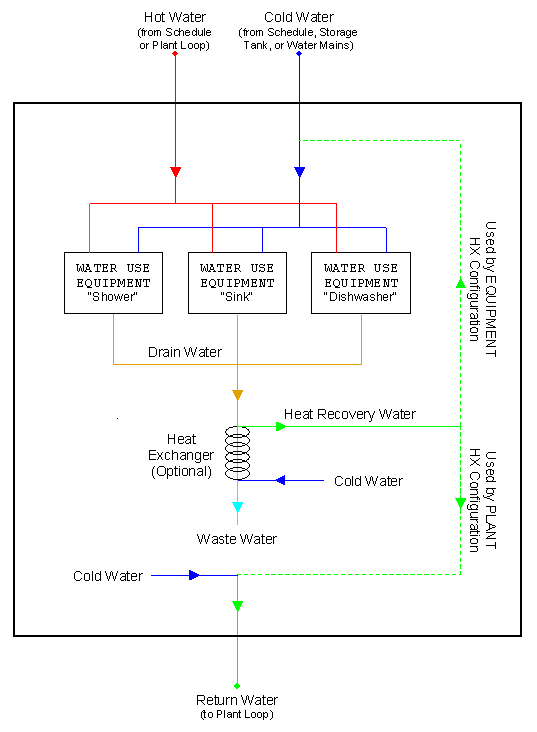
\includegraphics[width=0.9\textwidth, height=0.9\textheight, keepaspectratio=true]{media/image579.png}
\caption{Diagram of internal connections for WaterUse:Connections \protect \label{fig:diagram-of-internal-connections-for-wateruse}}
\end{figure}

The WaterUse:Connections object can be used stand-alone or coupled into a plant loop. In stand-alone mode, the Hot and Cold Water Supply Temperature Schedules override the values for the listed \hyperref[wateruseequipment]{WaterUse:Equipment} objects. When coupled to the plant, the Hot Water Supply Temperature Schedule is overridden by the actual plant loop inlet water temperature. When coupled to the plant, the WaterUse:Connections object should be on a \hyperref[branch]{Branch} object whose control type is set to Active.

\subsubsection{Inputs}\label{inputs-1-050}

\paragraph{Field: Name}\label{field-name-1-048}

The unique object name for reference by other objects.

\paragraph{Field: Inlet Node Name}\label{field-inlet-node-name-008}

The hot water inlet node when connected to a plant loop. The hot water supplies all of the \hyperref[wateruseequipment]{WaterUse:Equipment} objects that demand hot water. Insufficient supply temperature or flow results in cooler water at the tap.

\paragraph{Field: Outlet Node Name}\label{field-outlet-node-name-009}

The cold water outlet node, i.e.~the cold water supply mains, when connected to a plant loop. The return node provides make-up water for the hot water lost down the drain.

\paragraph{Field: Supply Water Storage Tank Name}\label{field-supply-water-storage-tank-name-002}

Reference to the \hyperref[waterusestorage]{WaterUse:Storage} object that supplies cold water to the listed \hyperref[wateruseequipment]{WaterUse:Equipment} objects. If the field is blank, or the tank is empty, fresh water is supplied from the water mains.

\paragraph{Field: Reclamation Water Storage Tank Name}\label{field-reclamation-water-storage-tank-name}

Reference to the \hyperref[waterusestorage]{WaterUse:Storage} object that stores the resulting graywater from the listed \hyperref[wateruseequipment]{WaterUse:Equipment} objects. If the field is blank, the graywater is not reclaimed.

\paragraph{Field: Hot Water Supply Temperature Schedule Name}\label{field-hot-water-supply-temperature-schedule-name-1}

Reference to the schedule object specifying the hot water temperature {[}C{]}. If blank in stand-alone mode, the hot water supply temperature defaults to the cold water supply temperature. This field (even if blank) overrides the Hot Water Supply Temperature Schedule in all of the listed \hyperref[wateruseequipment]{WaterUse:Equipment} objects.

\paragraph{Field: Cold Water Supply Temperature Schedule Name}\label{field-cold-water-supply-temperature-schedule-name-1-000}

Reference to the schedule object specifying the cold water temperature {[}C{]} from the supply mains that provides the cold water to the tap and makes up for all water lost down the drain. If blank, water temperatures are calculated by the \hyperref[sitewatermainstemperature]{Site:WaterMainsTemperature} object.

This field (even if blank) overrides the Cold Water Supply Temperature Schedule in all of the listed \hyperref[wateruseequipment]{WaterUse:Equipment} objects.

\paragraph{Field: Drain Water Heat Exchanger Type}\label{field-drain-water-heat-exchanger-type}

The heat exchanger type to be used for drainwater heat recovery. None indicates no heat recovery is to be simulated. Ideal sets a heat exchanger effectiveness of 1.0. Effectiveness is calculated dynamically for CounterFlow and CrossFlow options.

One popular type of drainwater heat exchanger is the Gravity-Film Heat Exchanger (GFX). The GFX is most closely approximated with the CounterFlow option, but keep in mind that the UA varies more with flow rate for the GFX than for most traditional heat exchangers.

\paragraph{Field: Drain Water Heat Exchanger Destination}\label{field-drain-water-heat-exchanger-destination}

The heat exchanger configuration to be used for drainwater heat recovery. The configuration determines where the heat will be used after it is recovered.

Plant indicates that the all of the recovered heat will be sent to the return flow at the outlet node of the WaterUse:Connections object to preheat the make-up cold water from the water mains.

Equipment indicates that the all of the recovered heat will be used to preheat the cold water flow side of the \hyperref[wateruseequipment]{WaterUse:Equipment} objects listed \emph{in this} WaterUse:Connections object

PlantAndEquipment indicates the recovered heat will be divided between the plant and the \hyperref[wateruseequipment]{WaterUse:Equipment} objects, as described above. This is the only option where the flow rates are equal in the drain and the heat exchanger.

\paragraph{Field: Drain Water Heat Exchanger U-Factor Times Area}\label{field-drain-water-heat-exchanger-u-factor-times-area}

The UA is the heat transfer coefficient {[}W/K{]} for the heat exchanger and is the product of U, the overall heat transfer coefficient, and A, the heat exchanger surface area.

\paragraph{Field: Water Use Equipment 1-10 Name}\label{field-water-use-equipment-1-10-name}

References to \hyperref[wateruseequipment]{WaterUse:Equipment} objects.

IDF examples:

\begin{lstlisting}

WaterUse:Connections,
  Domestic Water Uses,   !- Name
  Water Eq Inlet Node,   !- Inlet Node Name
  Water Eq Outlet Node, !- Outlet Node Name
  Rainwater Storage,   !- Supply Water Storage Tank Name
  Graywater Storage,   !- Reclamation Water Storage Tank Name
  ,   !- Hot Water Supply Temperature Schedule Name
  ,   !- Cold Water Supply Temperature Schedule Name
  CounterFlow,   !- Drain Water Heat Exchanger Type
  Plant,   !- Drain Water Heat Exchanger Destination
  1500,   !- Drain Water Heat Exchanger U-Factor Times Area {W/K}
  Sinks,   !- Water Use Equipment 1 Name
  Showers,   !- Water Use Equipment 2 Name
  Dishwasher,   !-   Water Use Equipment 3 Name
  Clotheswasher;   !- Water Use Equipment 4 Name
\end{lstlisting}

\subsubsection{Outputs}\label{outputs-1-031}

The following output variables are reported for the WaterUse:Connections object:

\begin{itemize}
\item
  HVAC,Average,Water Use Connections Hot Water Mass Flow Rate {[}kg/s{]}
\item
  HVAC,Average,Water Use Connections Cold Water Mass Flow Rate {[}kg/s{]}
\item
  HVAC,Average,Water Use Connections Total Mass Flow Rate {[}kg/s{]}
\item
  HVAC,Average,Water Use Connections Drain Water Mass Flow Rate {[}kg/s{]}
\item
  HVAC,Average,Water Use Connections Heat Recovery Mass Flow Rate {[}kg/s{]}
\item
  HVAC,Average,Water Use Connections Hot Water Volume Flow Rate {[}m3/s{]}
\item
  HVAC,Average,Water Use Connections Cold Water Volume Flow Rate {[}m3/s{]}
\item
  HVAC,Average,Water Use Connections Total Volume Flow Rate {[}m3/s{]}
\item
  HVAC,Sum,Water Use Connections Hot Water Volume {[}m3{]}
\item
  HVAC,Sum,Water Use Connections Cold Water Volume {[}m3{]}
\item
  HVAC,Sum,Water Use Connections Total Volume {[}m3{]}
\item
  HVAC,Average,Water Use Connections Hot Water Temperature {[}C{]}
\item
  HVAC,Average,Water Use Connections Cold Water Temperature {[}C{]}
\item
  HVAC,Average,Water Use Connections Drain Water Temperature {[}C{]}
\item
  HVAC,Average,Water Use Connections Return Water Temperature {[}C{]}
\item
  HVAC,Average,Water Use Connections Waste Water Temperature {[}C{]}
\item
  HVAC,Average,Water Use Connections Heat Recovery Water Temperature {[}C{]}
\item
  HVAC,Average,Water Use Connections Heat Recovery Effectiveness {[]}
\item
  HVAC,Average,Water Use Connections Heat Recovery Rate {[}W{]}
\item
  HVAC,Sum,Water Use Connections Heat Recovery Energy {[}J{]}
\item
  HVAC,Sum,Water Use Connections Plant Hot Water Energy {[}J{]}
\end{itemize}

\paragraph{Water Use Connections Hot Water Mass Flow Rate {[}kg/s{]}}\label{water-use-connections-hot-water-mass-flow-rate-kgs}

The mass flow rate of hot water supplied to all equipment, in units of kilograms per second (kg/s).

\paragraph{Water Use Connections Cold Water Mass Flow Rate {[}kg/s{]}}\label{water-use-connections-cold-water-mass-flow-rate-kgs}

The mass flow rate of cold water supplied to all equipment, in units of kilograms per second (kg/s).

\paragraph{Water Use Connections Total Mass Flow Rate {[}kg/s{]}}\label{water-use-connections-total-mass-flow-rate-kgs}

The total mass flow rate of water (hot + cold) supplied to all equipment, in units of kilograms per second (kg/s).

\paragraph{Water Use Connections Drain Water Mass Flow Rate {[}kg/s{]}}\label{water-use-connections-drain-water-mass-flow-rate-kgs}

The mass flow rate of drainwater from all equipment, in units of kilograms per second (kg/s).

\paragraph{Water Use Connections Heat Recovery Mass Flow Rate {[}kg/s{]}}\label{water-use-connections-heat-recovery-mass-flow-rate-kgs}

The mass flow rate of make-up water in the heat exchanger, in units of kilograms per second (kg/s).

\paragraph{Water Use Connections Hot Water Volume Flow Rate {[}m3/s{]}}\label{water-use-connections-hot-water-volume-flow-rate-m3s}

The volumetric flow rate of hot water supplied to all equipment and consumed down the drain, in units of cubic meters per second (m\(^{3}\)/s).

\paragraph{Water Use Connections Cold Water Volume Flow Rate {[}m3/s{]}}\label{water-use-connections-cold-water-volume-flow-rate-m3s}

The volumetric flow rate of cold water supplied to all equipment and consumed down the drain, in units of cubic meters per second (m\(^{3}\)/s).

\paragraph{Water Use Connections Total Volume Flow Rate {[}m3/s{]}}\label{water-use-connections-total-volume-flow-rate-m3s}

The total volumetric flow rate of water (hot + cold) supplied to all equipment and consumed down the drain, in units of cubic meters per second (m\(^{3}\)/s).

\paragraph{Water Use Connections Hot Water Volume {[}m3{]}}\label{water-use-connections-hot-water-volume-m3}

The volume of hot water supplied to all equipment and consumed down the drain, in units of cubic meters (m\(^{3}\)).

\paragraph{Water Use Connections Cold Water Volume {[}m3{]}}\label{water-use-connections-cold-water-volume-m3}

The volume of cold water supplied to all equipment and consumed down the drain, in units of cubic meters (m\(^{3}\)).

\paragraph{Water Use Connections Total Volume {[}m3{]}}\label{water-use-connections-total-volume-m3}

The total volume of water (hot+cold) supplied to all equipment and consumed down the drain, in units of cubic meters (m\(^{3}\)).

\paragraph{Water Use Connections Hot Water Temperature {[}C{]}}\label{water-use-connections-hot-water-temperature-c}

The temperature of hot water supplied to all equipment, in units of degrees Celsius (C).

\paragraph{Water Use Connections Cold Water Temperature {[}C{]}}\label{water-use-connections-cold-water-temperature-c}

The temperature of cold water supplied to all equipment, in units of degrees Celsius (C).

\paragraph{Water Use Connections Drain Water Temperature {[}C{]}}\label{water-use-connections-drain-water-temperature-c}

The water temperature at the drain equal to the mixed water temperature minus any heat losses to the zone, in units of degrees Celsius (C).

\paragraph{Water Use Connections Return Water Temperature {[}C{]}}\label{water-use-connections-return-water-temperature-c}

The temperature of make-up water returned to the plant loop, in units of degrees Celsius (C).

\paragraph{Water Use Connections Waste Water Temperature {[}C{]}}\label{water-use-connections-waste-water-temperature-c}

The temperature of the water leaving the heat exchanger. If no heat exchanger, the waste water temperature equals the drain water temperature, in units of degrees Celsius (C).

\paragraph{Water Use Connections Heat Recovery Water Temperature {[}C{]}}\label{water-use-connections-heat-recovery-water-temperature-c}

The temperature of the water leaving the heat exchanger. If no heat exchanger, the waste water temperature equals the drain water temperature, in units of degrees Celsius (C).

\paragraph{Water Use Connections Heat Recovery Effectiveness {[]}}\label{water-use-connections-heat-recovery-effectiveness}

The effectiveness value of the heat exchanger. The units are dimensionless.

\paragraph{Water Use Connections Heat Recovery Rate {[}W{]}}\label{water-use-connections-heat-recovery-rate-w}

The heat recovered by the heat exchanger and used to preheat the cold make-up water, in units of watts (W).

\paragraph{Water Use Connections Heat Recovery Energy {[}J{]}}\label{water-use-connections-heat-recovery-energy-j}

The energy recovered by the heat exchanger and used to preheat the cold make-up water, in units of Joules (J).

\paragraph{Water Use Connections Plant Hot Water Energy {[}J{]}}\label{water-use-connections-plant-hot-water-energy-j}

The plant loop energy consumed by the hot water used, in units of Joules (J). This output is also added to a meter with Resource Type = PlantLoopHeatingDemand, End Use Key = WaterSystems, and Group Key = Plant (ref. Output Meter).

\subsection{WaterUse:Storage}\label{waterusestorage}

The WaterUse:Storage object is a central component for complex water systems. This object is not needed if the only use of water is directly from the mains, or utility service water. If the building model is to include any on-site collection or wells or storing and reuse of graywater, then a WaterUse:Storage is needed. Each WaterUse:Storage can serve as a central node and make connections to numerous sources of supply or numerous components with demand. If a maximum capacity is not specified, the tank is assumed to have unlimited capacity. This is useful for sizing.

Storage tanks may handle a lot of water but show no use. This is because water usage is metered at the component level were water is used up. The only water a storage tank might use up is overflow water if it is discarded.

\subsubsection{Inputs}\label{inputs-2-046}

\paragraph{Field: Name}\label{field-name-2-043}

The unique object name for reference by other objects.

\paragraph{Field: Water Quality Subcategory}\label{field-water-quality-subcategory}

Describes the quality of the water contained in the tank. Used for reporting and to check that the uses and supply match the category of water quality.

\paragraph{Field: Maximum Capacity}\label{field-maximum-capacity}

The maximum volumetric capacity {[}m3{]} of the water tank. If blank, this field defaults to unlimited capacity.

\paragraph{Field: Initial Volume}\label{field-initial-volume}

The volume of water in the storage tank at the beginning of each simulation environmental period {[}m3{]}. This provides a starting point for the amount of water in storage.

\paragraph{Field: Design In Flow Rate}\label{field-design-in-flow-rate}

The design flow rate {[}m3/s{]} of fittings that provide water into the tank from external sources. In a scenario where a heavy rain fall is being harvested, the actual reclamation rate might be limited by pipe size or filtration. If blank, this field defaults to unlimited rate.

\paragraph{Field: Design Out Flow Rate}\label{field-design-out-flow-rate}

The design flow rate {[}m3/s{]} of fitting that withdraw water from the tank to end uses. Heavy demand (landscaping?) might be limited by pipe size or filtration. If Blank, this field defaults to unlimited rate.

\paragraph{Field: Overflow Destination}\label{field-overflow-destination}

Name of a second WaterUse:Storage that would receive overflow. Overflow could occur if the maximum capacity is reached or if the design in flow rate is exceeded. If left blank, then the overflow is discarded and lost from the water system.

\paragraph{Field: Type of Supply Controlled by Float Valve}\label{field-type-of-supply-controlled-by-float-valve}

The storage tank can include the capability of modeling a float valve that will call for water to be added to the tank. This field is used to select the type of system used to respondto fill requests made by a float valve. The available options are None , Mains , GroundwaterWell , or OtherTank. The float valve settings are described in the next two fields.

\paragraph{Field: Float Valve On Capacity}\label{field-float-valve-on-capacity}

The volumetric capacity {[}m3{]} of the water tank when a floating valve would turn on to allow filling the tank.

\paragraph{Field: Float Valve Off Capacity}\label{field-float-valve-off-capacity}

The volumetric capacity {[}m3{]} of the water tank when a floating valve would turn off after having been filling the tank.

\paragraph{Field: Backup Mains Capacity}\label{field-backup-mains-capacity}

The volumetric capacity of the tank that indicates where a secondary float valve will maintain the volume by calling for mains water. Used if the well or other tank cannot keep up with the needs of the main float valve. If left blank or equal 0.0, then there is no mains water backup. If specified, then mains water will be drawn once the storage tank reaches this level and then the mains water will fill all the way to capacity specified in the previous field.

\paragraph{Field: Other Tank Name}\label{field-other-tank-name}

This field contains the name of another WaterUse:Storage defined elsewhere in the input file. This field is only used if the Type of Controlled Supply field is set to OtherTank and the current tank is to be configured to be supplied by a second tank in response to a float valve.

\paragraph{Field: Water Thermal Mode}\label{field-water-thermal-mode}

Controls the method of determining the temperature of the water in the storage tank. The only available option at the current time is ScheduledTemperature.

\paragraph{Field: Water Temperature Schedule Name}\label{field-water-temperature-schedule-name-000}

Reference to the schedule object specifying the temperature {[}C{]} of the water in the tank. This takes the place of a full thermal model of the tank.

\paragraph{Field: Ambient Temperature Indicator}\label{field-ambient-temperature-indicator-001}

Reserved for future use. The field can be Schedule, Zone, or Outdoors.

\paragraph{Field: Ambient Temperature Schedule Name}\label{field-ambient-temperature-schedule-name-002}

Reserved for future use. Schedule name for ambient temperature when previous field is Schedule.

\paragraph{Field: Zone Name}\label{field-zone-name-1-010}

Reserved for future use. Name of zone where the tank is located.

\paragraph{Field: Tank Surface Area}\label{field-tank-surface-area}

Reserved for future zone thermal model.

\paragraph{Field: Tank U Value}\label{field-tank-u-value}

Reserved for future zone thermal model.

\paragraph{Field: Tank Outside Surface Material Name}\label{field-tank-outside-surface-material-name}

Reserved for future zone thermal model.

IDF examples:

\begin{lstlisting}

WaterUse:Storage,
  Tower 2 water tank, !- Name
  Tower water make up Holding tank, !- Water Quality Subcategory
  30.0 , !- Maximum Capacity {m3}
  10.0 , !- Initial Volume   {m3}
  20.0, !- Design In Flow Rate {m3}
  20.0, !- Design Out Flow Rate {m3}
  ,   !- Overflow Destination
  Mains, !- Type of Supply Controlled by Float Valve
  8.0 , !- Float Valve On Capacity {m3}
  10.0,   !- Float Valve Off Capacity {m3}
  3.0, !- Backup Mains Capacity {m3}
  ,   !- Other Tank Name
  ScheduledTemperature , !- Water Thermal Mode
  Water Tank Temp Sched , !- Water Temperature Schedule Name
  , !- Ambient Temperature Indicator
  , !- Ambient Temperature Schedule Name
  , !- Zone Name
  , !- Tank Surface Area {m2}
  , !- Tank U Value {W/m2-K}
  ; !- Tank Outside Surface Material Name
\end{lstlisting}

\subsubsection{Outputs}\label{outputs-2-026}

The following output variables are available for reporting for each WaterUse:Storage object.

\begin{itemize}
\item
  HVAC,Average,Water System Storage Tank Volume {[}m3{]}
\item
  HVAC,Average,Water System Storage Tank Net Volume Flow Rate {[}m3/s{]}
\item
  HVAC,Average,Water System Storage Tank Inlet Volume Flow Rate {[}m3/s{]}
\item
  HVAC,Average,Water System Storage Tank Outlet Volume Flow Rate {[}m3/s{]}
\item
  HVAC,Sum,Water System Storage Tank Mains Water Volume {[}m3{]}
\item
  HVAC,Average,Water System Storage Tank Mains Water Volume Flow Rate {[}m3/s{]}
\item
  HVAC,Average,Water System Storage Tank Water Temperature {[}C{]}
\item
  HVAC,Average,Water System Storage Tank Overflow Volume Flow Rate {[}m3/s{]}
\item
  HVAC,Sum,Water System Storage Tank Overflow Water Volume {[}m3{]}
\item
  HVAC,Average,Water System Storage Tank Overflow Temperature {[}C{]}
\end{itemize}

\paragraph{Water System Storage Tank Volume {[}m3{]}}\label{water-system-storage-tank-volume-m3}

This is the volume of water stored in the storage tank, in units of cubic meters (m\(^{3}\)).

\paragraph{Water System Storage Tank Net Volume Flow Rate {[}m3{]}}\label{water-system-storage-tank-net-volume-flow-rate-m3}

This is the net rate of flows in and out of the storage tank, in units of cubic meters (m\(^{3}\)).

\paragraph{Water System Storage Tank Inlet Volume Flow Rate {[}m3/s{]}}\label{water-system-storage-tank-inlet-volume-flow-rate-m3s}

This is the rate of flows into the storage tank, in units of cubic meters per second (m\(^{3}\)/s).

\paragraph{Water System Storage Tank Outlet Volume Flow Rate {[}m3{]}}\label{water-system-storage-tank-outlet-volume-flow-rate-m3}

This is the rate of flows out of the storage tank, in units of cubic meters (m\(^{3}\)).

\paragraph{Water System Storage Tank Mains Water Volume {[}m3{]}}\label{water-system-storage-tank-mains-water-volume-m3}

This is the volume of water drawn from the mains in order to fill the tank, in units of cubic meters per second (m\(^{3}\)/s). This output is also added to a meter with Resource Type = MainsWater, End Use Key = WaterSystem, and Group Key = System. The water quality sub-category may be entered as any type (defined in WaterUse:Storage object input for Water Quality Subcategory) (ref. Output Meter).

\paragraph{Water System Storage Tank Mains Water Volume Flow Rate {[}m3/s{]}}\label{water-system-storage-tank-mains-water-volume-flow-rate-m3s}

This is the rate of water draw from the mains in order to fill the tank, in units of cubic meters per second (m\(^{3}\)/s).

\paragraph{Water System Storage Tank Water Temperature {[}C{]}}\label{water-system-storage-tank-water-temperature-c}

This is the temperature of the water in the tank, in units of degrees Celsius (C).

\paragraph{Water System Storage Tank Overflow Volume Flow Rate {[}m3/s{]}}\label{water-system-storage-tank-overflow-volume-flow-rate-m3s}

This is the rate of water flows that overflow the tank either because of limits on how fast the tank can fill or because the tank is full and cannot handle the water provided, in units of cubic meters per seconc (m\(^{3}\)/s).

\paragraph{Water System Storage Tank Overflow Water Volume {[}m3{]}}\label{water-system-storage-tank-overflow-water-volume-m3}

This is the volume of water overflowing the tank because of limits on how fast the tank can fill or because the tank is full and cannot handle the water provided, in units of cubic meters (m\(^{3}\)).

\paragraph{Water System Storage Tank Overflow Temperature {[}C{]}}\label{water-system-storage-tank-overflow-temperature-c}

This the temperature of overflow water leaving the tank.

\subsection{WaterUse:RainCollector}\label{wateruseraincollector}

The WaterUse:RainCollector object is used for harvesting rainwater falling on building surfaces. The rainwater is sent to a \hyperref[waterusestorage]{WaterUse:Storage} object. In order to use this object it is necessary to also include a \hyperref[siteprecipitation]{Site:Precipitation} object to describe the rates of rainfall.

\subsubsection{Inputs}\label{inputs-3-041}

\paragraph{Field: Name}\label{field-name-3-037}

The unique object name for reference by other objects.

\paragraph{Field: Storage Tank Name}\label{field-storage-tank-name}

A reference to a \hyperref[waterusestorage]{WaterUse:Storage} object where the rainwater will be collected and stored for later use.

\paragraph{Field: Loss Factor Mode}\label{field-loss-factor-mode}

The WaterUse:RainCollector model includes a loss factor that indicates the portion of incident rain that is not successfully collected. Two modes are available: Constant and Scheduled. Enter Constant in this field for the model to use a simple fixed loss factor defined in the next field. For versatility, the loss factor can follow a schedule by entering Scheduled in this field and then the name of a schedule in the second field below.

\paragraph{Field: Collection Loss Factor}\label{field-collection-loss-factor}

Constant loss factor for how much of the incident rainwater is lost and not collected. The factor should be between 0 and 1.

\paragraph{Field: Collection Loss Factor Schedule Name}\label{field-collection-loss-factor-schedule-name}

Name of a schedule that defines a variable collection loss factor if the mode is selected as Scheduled.

\paragraph{Field: Maximum Collection Rate}\label{field-maximum-collection-rate}

The maximum flow rate {[}m3/s{]} for rainwater collection. In a scenario where a heavy rain fall is being harvested, the actual reclamation rate might be limited by pipe size or the filtration system.

\paragraph{Field: Collection Surface 1-10 Name}\label{field-collection-surface-1-10-name}

A reference to the name of a surface object which will collect the rain. Typically the collection surfaces would correspond to roof surfaces on the building. The effective area for rainwater collection is the horizontal component (area * cosine of the slope, etc.). More detailed modeling of rainwater collection can be added later to account for factors such as wind speed and direction, etc.

IDF examples:

\begin{lstlisting}

WaterUse:RainCollector,
  My Test Rain Collector ,!- Name
  My Test Tank ,   !-   Storage Tank Name
  CONSTANT,   !- Loss Factor Mode
  0.9 ,   !- Collection Loss Factor
  ,   !- Collection Loss Factor Schedule Name
  1.0 ,   !- Maximum Collection Rate
  SouthRoof ,   !- Collection Surface 1 Name
  NorthRoof1,   !- Collection Surface 2 Name
  NorthRoof3 ,   !- Collection Surface 3 Name
  NorthRoof2 ;   !- Collection Surface 4 Name
\end{lstlisting}

\subsubsection{Outputs}\label{outputs-3-023}

\begin{itemize}
\item
  HVAC,Average,Water System Rainwater Collector Volume Flow Rate {[}m3/s{]}
\item
  HVAC,Sum,Water System Rainwater Collector Volume {[}m3{]}
\end{itemize}

\paragraph{Water System Rainwater Collector Volume Flow Rate {[}m3/s{]}}\label{water-system-rainwater-collector-volume-flow-rate-m3s}

This output variable provides the rate of water collected by the WaterUse:RainCollector, in units of cubic meters per second (m\(^{3}\)/s).

\paragraph{Water System Rainwater Collector Volume {[}m3{]}}\label{water-system-rainwater-collector-volume-m3}

This output variable provides the volume of water collected by the WaterUse:RainCollector, in units of cubic meters per second (m\(^{3}\)/s). This output is also added to a meter with Resource Type = OnSiteWater, End Use Key = RainWater, and Group Key = System (ref. Output Meter).

\subsection{WaterUse:Well}\label{waterusewell}

The WaterUse:Well object is for simulating on-site water supply from a well. Well water is pumped out of the ground and into a \hyperref[waterusestorage]{WaterUse:Storage}. The operation of the ground water well is controlled by the associated \hyperref[waterusestorage]{WaterUse:Storage} which is assumed to be operated as a vented cistern with no pressure tank. The current implementation is very simple and only requires two numeric inputs: the rated pump flow and power. A more elaborate well model may be added and many input fields are reserved for this future expansion.

\subsubsection{Inputs}\label{inputs-4-038}

\paragraph{Field: Name}\label{field-name-4-033}

Unique name of this well.

\paragraph{Field: Storage Tank Name}\label{field-storage-tank-name-1}

A reference to a \hyperref[waterusestorage]{WaterUse:Storage} object where the rainwater will be collected and stored for later use.

\paragraph{Field: Pump Depth}\label{field-pump-depth}

Reserved for future use. Effective depth of well {[}m{]}

\paragraph{Field: Pump Rated Flow Rate}\label{field-pump-rated-flow-rate}

This is the nominal pump flow rate {[}m3/s{]}. This field is required.

\paragraph{Field: Pump Rated Head}\label{field-pump-rated-head}

Reserved for future use {[}Pa{]}. Pump head at rated conditions in Pascals.

\paragraph{Field: Pump Rated Power Consumption}\label{field-pump-rated-power-consumption}

This is the pump power at the nominal pump flow rate {[}W{]}. This field is required.

\paragraph{Field: Pump Efficiency}\label{field-pump-efficiency}

Reserved for future use.

\paragraph{Field: Well Recovery Rate}\label{field-well-recovery-rate}

Reserved for future use. Rate at which ground water enters well during a sustained draw, e.g., 2 hour well test {[}m3/s{]}.

\paragraph{Field: Nominal Well Storage Volume}\label{field-nominal-well-storage-volume}

Reserved for future use. Capacity in well after long period of inactivity and the usual water table depth. {[}m3{]}

\paragraph{Field: Water Table Depth Mode}\label{field-water-table-depth-mode}

Reserved for future use. Two options available: Constant or Scheduled

\paragraph{Field: Water Table Depth}\label{field-water-table-depth}

Reserved for future use. Depth of water table from \hyperref[waterusestorage]{WaterUse:Storage}

\paragraph{Field: Water Table Depth Schedule Name}\label{field-water-table-depth-schedule-name}

Reserved for future use.

An example input object:

\begin{lstlisting}

WaterUse:Well,
  My Test Well,   !- Name
  Tower 1 Water Tank,   !- Storage Tank Name
  ,   !- Pump Depth
  0.1,   !- Pump Rated Flow Rate {m3/s}
  ,   !- Pump Rated Head {Pa}
  120,   !- Pump Rated Power Consumption {W}
  ,   !- Pump Efficiency
  ,   !- Well Recovery Rate {m3/s}
  ,   !- Nominal Well Storage Volume {m3}
  ,   !- Water Table Depth Mode
  ,   !- Water Table Depth
  ;   !- Water Table Depth Schedule Name
\end{lstlisting}

\subsubsection{Outputs}\label{outputs-4-019}

The following output variables are available for reporting for each WaterUse:Well object.

\begin{itemize}
\item
  HVAC,Average,Water System Groundwater Well Requested Volume Flow Rate {[}m3/s{]}
\item
  HVAC,Average,Water System Groundwater Well Volume Flow Rate {[}m3/s{]}
\item
  HVAC,Sum,Water System Groundwater Well Volume {[}m3{]}
\item
  HVAC,Average,Water System Groundwater Well Pump Electric Power {[}W{]}
\item
  HVAC,Sum,Water System Groundwater Well Pump Electric Energy {[}J{]}
\end{itemize}

\paragraph{Water System Groundwater Well Requested Volume Flow Rate {[}m3/s{]}}\label{water-system-groundwater-well-requested-volume-flow-rate-m3s}

This is the volume flow rate that the water system requested from the well, in units of cubic meters per second (m\(^{3}\)/s).

\paragraph{Water System Groundwater Well Volume Flow Rate {[}m3/s{]}}\label{water-system-groundwater-well-volume-flow-rate-m3s}

This is the volume flow water of water actually obtained from the well, in units of cubic meters per second (m\(^{3}\)/s).

\paragraph{Water System Groundwater Well Volume {[}m3{]}}\label{water-system-groundwater-well-volume-m3}

This is the volume of water obtained from the well, in units of cubic meters (m\(^{3}\)). This output is also added to a meter with Resource Type = OnSiteWater, End Use Key = WellWater, and Group Key = System (ref. Output Meter).

\paragraph{Water System Groundwater Well Pump Electric Power {[}W{]}}\label{water-system-groundwater-well-pump-electric-power-w}

This is the electrical power of the pump used to extract water from the well, in units of watts (W).

\paragraph{Water System Groundwater Well Pump Electric Energy {[}J{]}}\label{water-system-groundwater-well-pump-electric-energy-j}

This is the electricity energy used by the pump to extract water from the well, in units of Joules (J). This output is also added to a meter with Resource Type = Electricity, End Use Key = WaterSystems, and Group Key = System (ref. Output Meter).
